\begin{figure}[htbp]
\centering
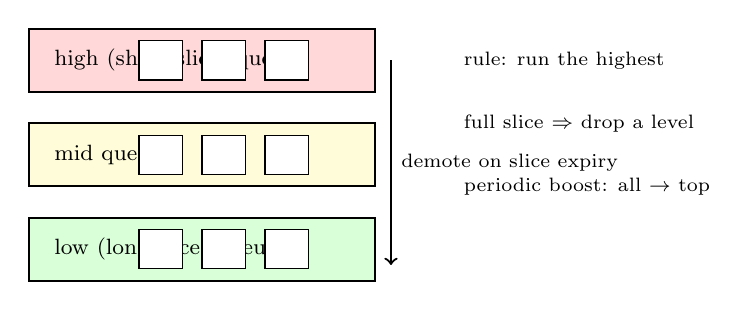
\begin{tikzpicture}[font=\footnotesize, x=1cm, y=1cm]
  \foreach \y/\pri/\fill in {3.4/{high (short slice)}/red!15,
                             2.2/{mid}/yellow!15,
                             1.0/{low (long slice)}/green!15} {
    \draw[thick,fill=\fill] (0,\y) rectangle (4.4,\y+0.8);
    \node[anchor=west] at (0.2,\y+0.4) {\pri\ queue};
    \foreach \x in {1.4,2.2,3.0} {
      \draw[fill=white] (\x,\y+0.15) rectangle (\x+0.55,\y+0.65); }
  }
  \draw[->,thick] (4.6,3.8) -- (4.6,1.2) node[midway,right]
    {\scriptsize demote on slice expiry};
  \node[anchor=west] at (5.4,3.8) {\scriptsize rule: run the highest};
  \node[anchor=west] at (5.4,3.0) {\scriptsize full slice $\Rightarrow$ drop a level};
  \node[anchor=west] at (5.4,2.2) {\scriptsize periodic boost: all $\to$ top};
\end{tikzpicture}
\caption{MLFQ without code: short jobs naturally fall to the bottom
(they finish before being demoted); long jobs sink and get long
slices; a periodic priority boost stops starvation. The policy
approximates STCF without knowing job lengths.}
\label{fig:mlfq12}
\end{figure}
